\chapter{Ergebnisse dieser Arbeit}

In diesem Kapitel werden die Funktionalitäten des Prototyps beschrieben. Zum Schluss werden die Kalkulationsergebnisse der Kostenanalyse als Tabelle und die Messungsergebnisse der Performance Messung als Liniendiagramm bereitgestellt und auf einzelne Ergebnisse eingegangen. Außerdem dient dieses Kapitel zur kurzen Übersicht über die Ergebnisse der Performance und Kosten. 

\section{Beschreibung und Funktionalität des Prototyps}

Der Prototyp hat die Funktionalität des Uploads und Downloads von Objekten nach S3 oder Cloud Storage. Der Nutzer kann sich zwischen AWS und GC entscheiden, indem die cloud\_provider Umgebungsvariable vor dem Ausführen des Programms gesetzt wird. Damit das Programm erfolgreich durchlaufen kann, müssen alle Umgebungsvariablen in der \verb|application.properties| Datei gesetzt werden. Außerdem wird eine Authentifizierung für GC und AWS verlangt, sonst schlägt das Programm fehl. Die Authentifizierung für GC kann über die ADC erfolgen. In der offiziellen Dokumentation werden die verschiedenen Methoden aufgelistet. Für den Prototypen wurde die lokale Entwicklungsumgebung für die Authentifizierung durch: 

\begin{lstlisting}
export GOOGLE\_APPLICATION\_CREDENTIALS=<jsonKeyPath>
\end{lstlisting}
	
	oder durch den \verb|gcloud| cli Befehl: 
	
\begin{lstlisting}
gcloud auth application-default login
\end{lstlisting}
	
	verwendet. Dabei ist der \verb|jsonKeyPath| der Pfad zum erstellten Service Account, welche Rechte für das Uploaden und Downloaden besitzt. Unter \url{https://cloud.google.com/docs/authentication/provide-credentials-adc} können die ADC Credentials Methoden eingesehen werden.\\
	
Für die Authentifizierung mit AWS benötigt es lediglich das AWS Toolkit Plugin. Dieses stellt AWS für einige IDEs zur Verfügung. Unter anderem für Visual Studio, Eclipse und Intellij Idea. Falls das AWS Toolkit nicht zur Verfügung steht, kann die Authentifizierung auch über die \verb|aws cli| erfolgen. Durch \verb|aws configure| können die Credentials gesetzt werden. Unter \url{https://docs.aws.amazon.com/sdk-for-java/latest/developer-guide/setup-basics.html} können die AWS Credentials Methoden eingesehen werden. Nachdem die Authentifizierungseinstellungen und die Umgebungsvariablen gesetzt wurden, kann das Programm gestartet werden. Damit die Dateien in der richtigen Speicherklasse hochgeladen werden, muss für GC der korrekte Bucket Name angegeben werden. In AWS muss jedoch die gewünschte Speicherklasse angegeben werden, damit das Objekt in diese geschrieben wird. Dieser Unterschied besteht, da in GC die Speicherklasse über die GC Konsole für ein Bucket ausgewählt werden kann. In AWS ist dies jedoch nicht möglich, deshalb haben alle Buckets in AWS bei Erstellung die Standard Speicherklasse eingestellt. Die Objektklasse muss speziell durch den Parameter \verb|storageClass| beim Hochladen angegeben werden. Das Objekt wird durch die SSE KMS verschlüsselt hochgeladen. Die Verschlüsselung wird automatisch von beiden Cloud Providern durchgeführt. Dabei muss der entsprechende KMS Schlüssel des ausgewählten Cloud Providers der Environment Variable \verb|sse_kms_key_id_arn| übergeben werden. Beim Herunterladen des Objekts muss dieser ARN Schlüssel erneut mitgegeben werden, damit das Objekt entschlüsselt werden kann. Die Hauptklasse \verb|HandsonAwsGcApplication| ruft die entsprechende Klasse für AWS oder GC auf und initialisiert diese. Vorher müssen die Parameter für die \verb|.uploadObject(bucketName, key, filePath, encryptionKey, storageClass)| und \verb|.getPresignedUrl(bucketName, key, minutes, encryptionKey)| übergeben werden. Die Minuten stellen die Zeit ein, in der die generierte signierte URL gültig ist. Der \verb|storageClass| Parameter gilt nur für die AWS Funktion und kann die Werte \verb|STANDARD, STANDARD_IA| und \verb|ONEZONE_IA| annehmen.\\

Über Terraform werden die Buckets erstellt und die Konfigurationen eingestellt. Diese Konfigurationen sind an die Anforderungen an leoticket angepasst. Die Buckets müssen vor dem Programmstart bereits existieren, deshalb muss die Terraform Datei am Anfang durchlaufen. Die Terraform Dateien werden im entsprechenden Ordner bereitgestellt. Diese werden vor dem Programmstart als erstes ausgeführt, um die benötigten Ressourcen zu erstellen.\\

Der Prototyp dient außerdem dazu, die APIs miteinander zu vergleichen und jeweils ähnliche Funktionalitäten für beide Provider bereitzustellen.

\newpage

\section{Zusammenfassung der Ergebnisse}

In diesem Abschnitt werden die Kosten der verschiedenen Speicherklassen nochmal aufgegriffen und die Gesamtkosten als Tabelle dargestellt. Auch werden die Messungsergebnisse der Performance Analyse als Liniendiagramm bereitgestellt und die Zahlen der Kosten und Messungen untersucht.

\subsection{Kalkulationsergebnisse}

Im folgenden werden die Gesamtkosten der Speicherklasse von beiden Cloud Providern dargestellt und untersucht. Zuerst werden in der unteren Tabelle die Kosten von AWS untersucht:

\begin{table}[!h]
\begin{tabular}{ |s|p{2cm}|p{2cm}|p{2cm}|p{2cm}| }
\hline
\rowcolor{blue!35}
 & \textbf{Standard} & \textbf{Intelligent Tiering} & \textbf{Standard-IA} & \textbf{One Zone-IA}\\
\hline
\textbf{Monatliche Speicherkosten} & 70.27 EUR & 70.27 EUR & 38.72 EUR & 30.98  EUR \\
\textbf{PUT Requests}   & 1.35 EUR & 1.35 EUR  & 2.50 EUR & 2.50 EUR\\
\textbf{GET Requests}  & 0.22 EUR & 0.22 EUR  & 0.50 EUR & 0.50 EUR\\
\textbf{Datenabrufe} & -- & -- & 0.47 EUR & 0.47 EUR\\
\hline
\textbf{Data Transfer} & \multicolumn{3}{c}{4.20 EUR} &\\
\hline
\textbf{Monitoring und Automation objects} & -- & 75.19 EUR & -- & --\\
\textbf{Gesamtkosten pro Monat(ohne Vorauszahlung)} & 76.04 EUR & 151.23 EUR & 46.39 EUR & 38.65 EUR\\
\hline
\textbf{Vorabzahlung} & 162.42 EUR & 162.42 EUR & 300.76 EUR & 300.76 EUR \\
\hline
\hline
\textbf{Gesamtkosten im ersten Monat} & \textbf{238.46 EUR} & \textbf{313.65 EUR} & \textbf{347.15 EUR} & \textbf{339.41 EUR}\\
\hline
\end{tabular}
\caption{Zusammenfassung der Gesamtkosten für AWS S3 pro Speicherklasse}
\end{table}

In dieser Tabelle werden in der letzten Zeile# die Gesamtkosten der Speicherklassen pro Monat veranschaulicht. Die Gesamtkosten im ersten Monat der Speicherklasse Standard beträgt 238.46 EUR. In diesen Kosten stecken die Vorabzahlung, die PUT und GET Request Gebühren und die Datenübertragungsgebühren. Im Intelligent Tiering und Standard sind die Datenabrufgebühren nicht enthalten, da dafür keine Gebühren abgezogen werden. Die Gesamtkosten des Intelligent Tiering pro Monat beträgt 313.65 EUR. Die Kosten des Intelligent Tiering hängen jedoch von der Speicherverteilung ab. Die Kosten sind grobe Werte und können von der Verteilung des Speichers in verschiedene Speicherklassen in Prozent abhängen. Bei der Standard-IA Speicherklasse sind es mit 347.15 EUR die teuersten Kosten im Vergleich zu den anderen Speicherklassen. Die One Zone-IA ist mit 339.41 EUR die billigste Speicherklasse.

\newpage        

In Google Cloud gibt es keine Vorabzahlungen im Gegensatz zu AWS. Hier unterscheiden sich die Gesamtkosten der verschiedenen Speicherklassen zu AWS. In der folgenden Tabelle werden die Gesamtkosten zusammengefasst:

\begin{table}[!h]
\centering
\begin{tabular}{ |s|p{2cm}|p{2cm}|p{2cm}| }
\hline
\rowcolor{green!25}
 & \textbf{Standard} & \textbf{Nearline} & \textbf{Coldline}\\
\hline
\textbf{Monatliche Speicherkosten} & 63.75 EUR & 36.03 EUR & 16.63 EUR\\
\textbf{Datenabrufe} & -- & 0.45 EUR & 0.90 EUR\\
\textbf{Klasse A Operationen}   & 1.21 EUR & 2.42 EUR  & 4.84 EUR\\
\textbf{Klasse B Operationen}  & 0.19 EUR & 0.48 EUR   & 4.84 EUR\\
\hline
\textbf{Internet Egress monatlich} & \multicolumn{2}{c}{3.83 EUR pro 0 bis 1TB} &\\
\hline
\hline
\textbf{Gesamtkosten pro Monat} & \textbf{68.98 EUR} & \textbf{43.21 EUR} & \textbf{31.04 EUR}\\
\hline
\end{tabular}
\caption{Zusammenfassung der Gesamtkosten für GC Storage pro Speicherklasse}
\end{table}

Die Gesamtkosten bestehen laut Tabelle hauptsächlich aus den Speicherkosten und die Internet Egress, ausgehend von GC zum Internet, beispielsweise beim Abrufen von Dateien. Es fallen keine Gebühren für die Datenabrufe der Standard Speicherklasse an. Die Gesamtkosten des Standards beträgt 68.98 Euro, der Nearline 43.21 Euro und des Coldline 31.04 Euro. 

\newpage
\subsection{Messergebnisse}

In diesem Abschnitt werden die Messergebnisse der Performance Analyse bereitgestellt. Die Speicherklassen Standard, Standard-IA und One Zone-IA von AWS wurden jeweils mit Standard, Nearline und Coldline von GC verglichen. Im folgenden werden die Ergebnisse der Upload Dauer aller Speicherklassen als Liniendiagramm dargestellt:

\begin{figure}[h]
	\centering
	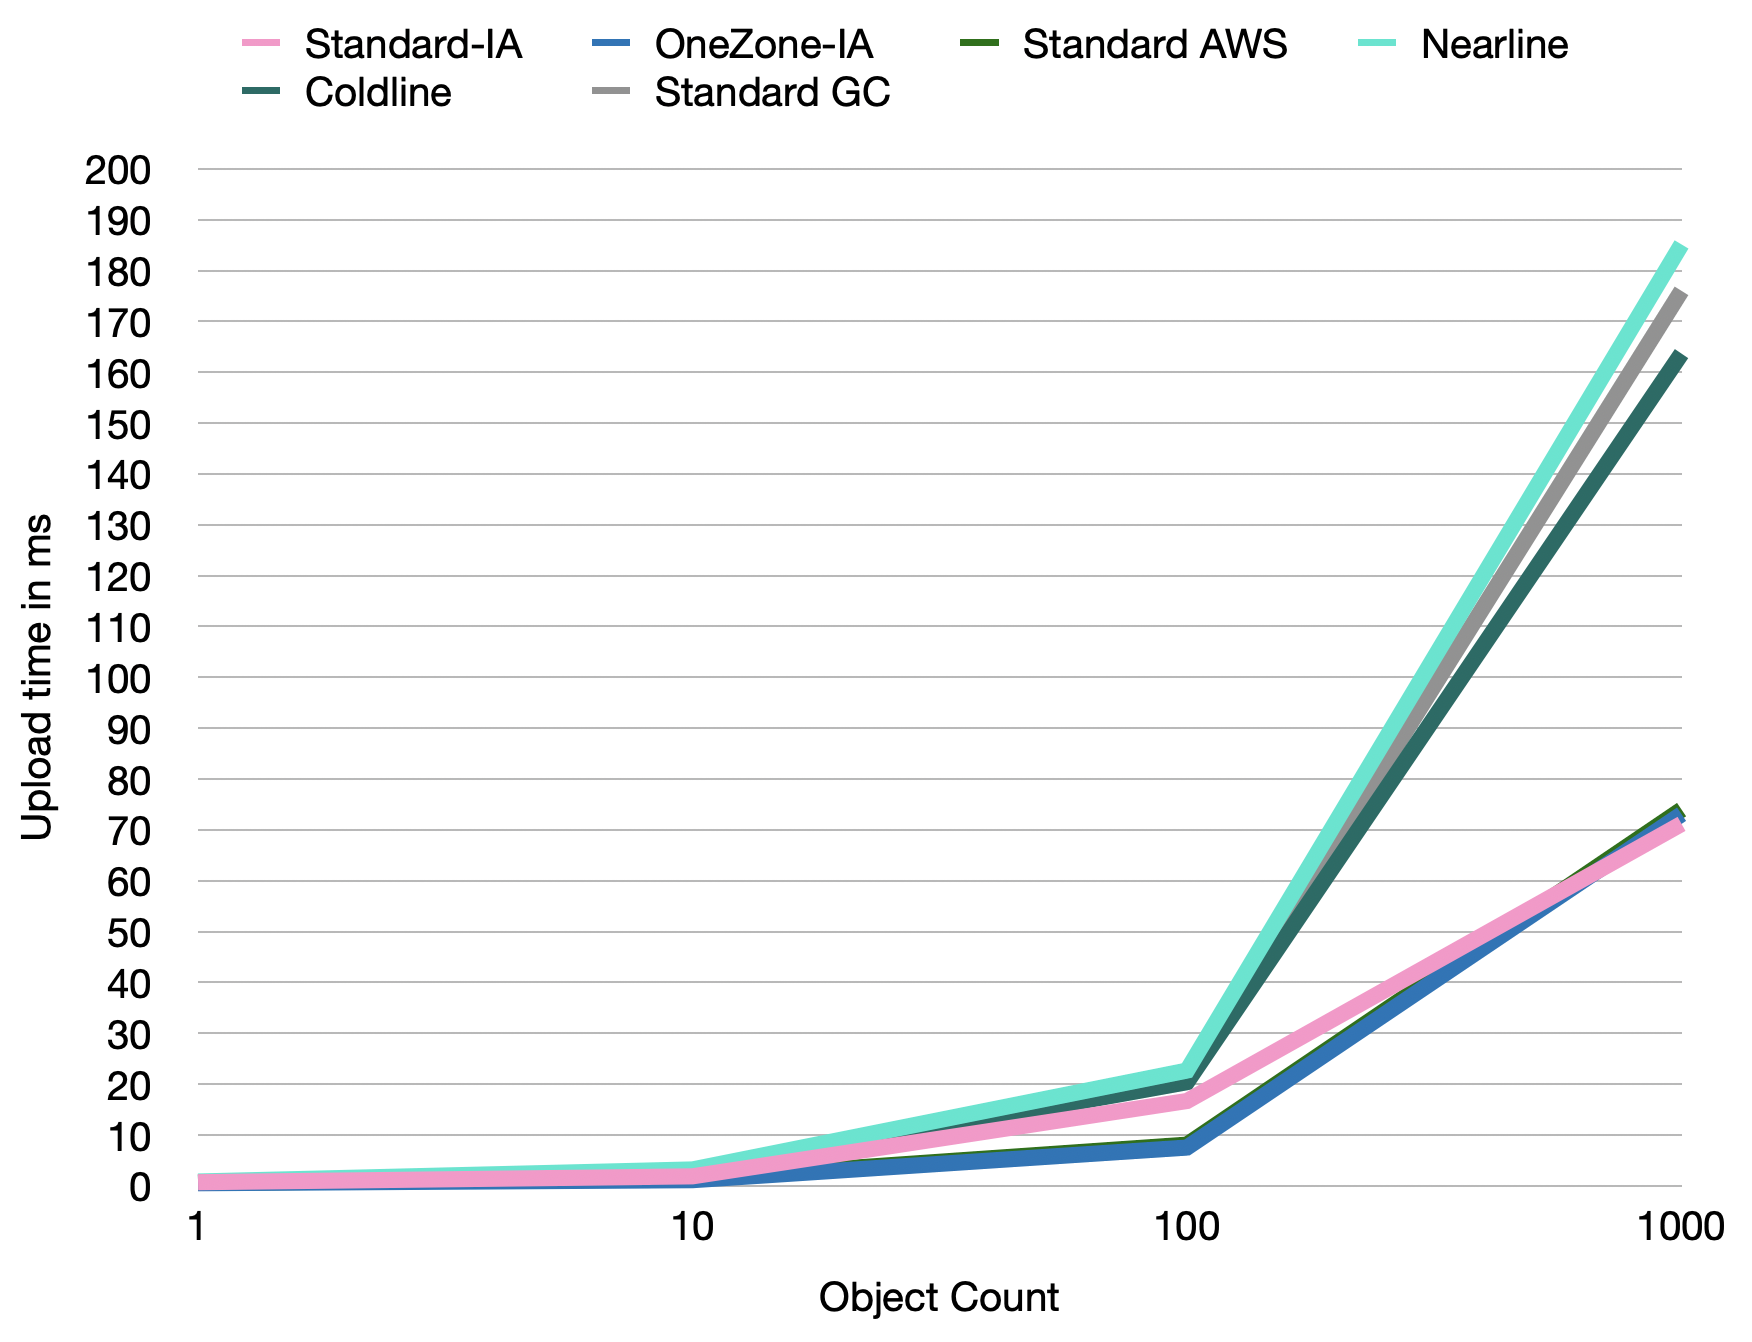
\includegraphics[width=14cm,keepaspectratio]{Pictures/UploadTime.png}
	\caption{Upload Zeit der verschiedenen Speicherklassen}
\end{figure}	

Die X-Achse beschreibt die Objektanzahl, die für jede Speicherklasse hochgeladen wurde. Die Farben unterscheiden die verschiedenen Speicherklassen, wobei die Speicherklassen von AWS jeweils nebeneinander platziert sind, genauso wie die Speicherklassen von GC. Die Zahlen vom Abschnitt 3.5.1 wurden in diesen Diagramm eingefügt, um die Unterschiede zwischen den Speicherklassen beider Provider zu visualisieren. So liegen die Speicherklassen von AWS im Graph nah beieinander, ähnlich wie jene von GC. Beim Hochladen von einer Datei bis hin zu zehn Dateien gibt es minimale Unterschiede. Diese Werte liegen unter 3 Sekunden. Die Linien gehen ab dem Hochladen von 11 bis 1000 Dateien stärker auseinander. Die drei Speicherklassen von GC entfernen sich von den drei Speicherklassen von AWS. Ab 100 Dateien gibt es erneut einen Knick und die Speicherklassen von GC entfernen sich weiter von den AWS Speicherklassen. Die GC Speicherklassen wachsen steiler nach oben als bei AWS und bewegen sich in höheren Sekunden Bereichen von ungefähr 20 bis hin zu 190 Sekunden. AWS bewegt sich dabei maximal bis 140 Sekunden. 

\newpage

Die Unterschied sind beim Download weniger stark ausgeprägt als beim Upload45, denn die Zahlen für den Download bewegen sich in Bereichen von 16 bis hin zu 1556 Millisekunden. Hier steigen die Werte nicht höher als 2 Sekunden. In der folgenden Abbildung wird dies veranschaulicht:

\begin{figure}[h]
	\centering
	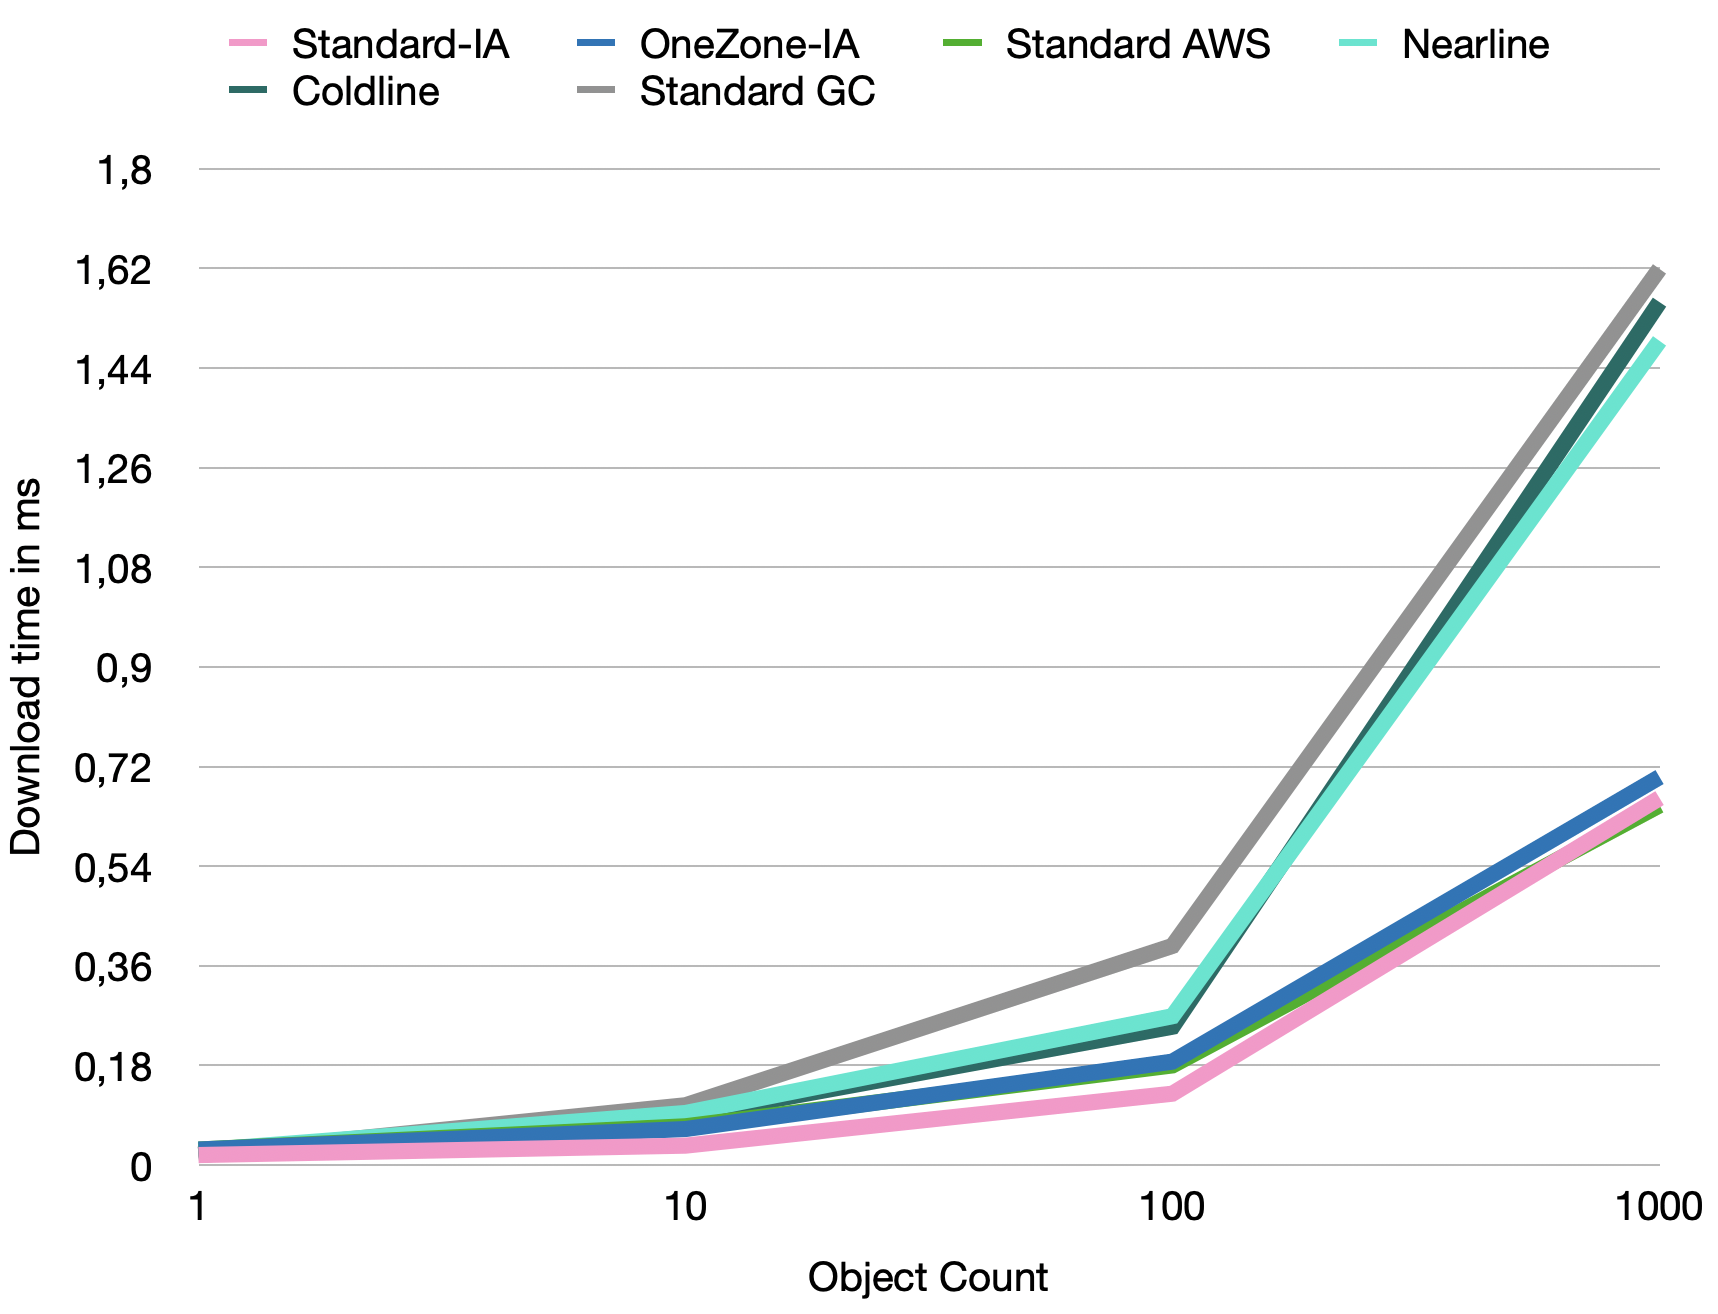
\includegraphics[width=14cm,keepaspectratio]{Pictures/DownloadTime.png}
	\caption{Download Zeit der verschiedenen Speicherklassen}
\end{figure}

Dieser Graph ähnelt dem Graph des Uploads in Abbildung 4.2.3. Denn auch hier entfernen sich die Linien der GC Speicherklassen von den AWS Speicherklassen. Ab Downloads von zehn Dateien trennen sich die Cloud Provider voneinander. Die Coldline Speicherklasse von GC hat dabei am längsten mit 1556 Millisekunden für den Download von 1000 Dateien gebraucht. Die schnellste Speicherklasse von AWS ist die OneZone-IA mit 569 Millisekunden beim Download von 1000 Dateien. Wobei die Speicherklassen von AWS nah beieinander liegen und weniger als 1 Sekunde für den Download gebraucht haben. Bei GC dauern die Downloads von 1000 Dateien mindestens 1500 Millisekunden. Im Bereich von einer bis zehn Dateien bewegen sich die Speicherklassen in unter 160 Millisekunden Bereichen. Jedoch gibt es bei zehn Dateien bereits erste minimale Unterschiede, die langsam wachsen.\\
 